A small ball with mass $M = 0.2$~kg rests on a vertical column with height
$h = 5$~m. A bullet with mass $m = 0.01$~kg, moving with velocity
$v_0 = 500$~m/s, passes horizontally through the center of the ball (Fig.~1).
The ball reaches the ground at a distance $s = 20$~m. Where does the bullet
reach the ground? What part of the kinetic energy of the bullet was converted
into heat when the bullet passed through the ball? Neglect resistance of the
air. Assume that $g = 10~\mathrm{m/s^2}$.

\begin{center}
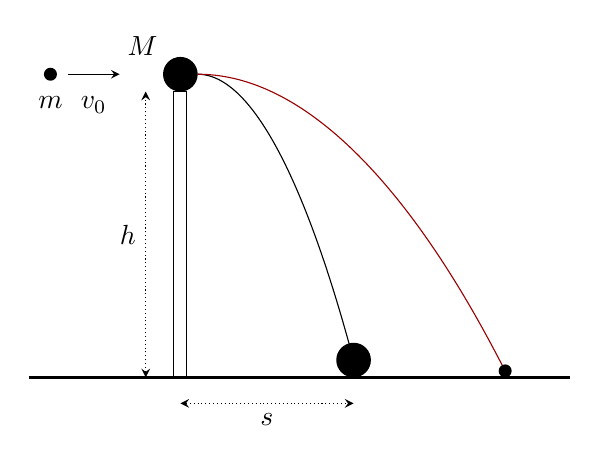
\begin{tikzpicture}[scale=0.55, >=stealth]
  \draw[thick] (-1.5,0) -- (11,0);
  \draw (1.85,0) rectangle (2.15,6.6);
  \fill (2,7) circle (0.4);
  \node[above left] at (1.7,7.2) {$M$};
  \fill (-1,7) circle (0.15);
  \draw[->] (-0.6,7) -- (0.6,7);
  \node[below] at (-1,6.7) {$m$};
  \node[below] at (0,6.7) {$v_0$};
  \draw[<->, densely dotted] (1.2,0) -- (1.2,6.6) node[midway, left] {$h$};
  \draw (2.4,7) parabola (6,0.4);
  \fill (6,0.4) circle (0.4);
  \draw[red!60!black] (2.4,7) parabola (9.5,0.15);
  \fill (9.5,0.15) circle (0.15);
  \draw[<->, densely dotted] (2,-0.6) -- (6,-0.6) node[midway, below] {$s$};
\end{tikzpicture}
\figcap{Fig.~1}
\end{center}
